\documentclass{article}
\usepackage{amsmath,amssymb}
\usepackage{float}
\usepackage{graphicx}
\usepackage{pdflscape}
% \usepackage{xcolor}
\usepackage[colorlinks=true,linkcolor=red]{hyperref}
\begin{document}

\subsection*{Jump Instruction}

In this architecture, the address bus and the program counter (PC) are both \textbf{8 bits}. 
The J-type instruction format stores an \textbf{8-bit target address}. Therefore, the jump 
instruction already contains the \textbf{complete address of the destination}. 

When a jump instruction is executed, the processor simply loads the target field into the PC.

\[
PC \leftarrow \text{TargetAddress}
\]

Unlike standard MIPS designs, no concatenation with the upper bits of $PC+4$ is required. 
In larger architectures the jump instruction stores fewer address bits, so the remaining 
bits are taken from the current PC. However, since the full 8-bit address space is already 
encoded in the instruction here, the target address can be used directly.

\bigskip

\subsection*{Branch Instruction and Sign Extension}

Branch instructions use a \textbf{4-bit immediate field} to represent the branch offset. 
Since the PC is \textbf{8 bits}, the immediate value must first be expanded to 8 bits before 
being used in address calculation. This process is called \textbf{sign extension}.

Sign extension preserves the sign of the number by copying the most significant bit (MSB) 
of the immediate value into the newly added higher bits. Thus, a 4-bit value is converted 
into an 8-bit signed number.

\[
\text{Immediate}_{8} = \text{SignExtend}(\text{Immediate}_{4})
\]

This allows the offset to represent both \textbf{forward and backward branches}. For example,

\[
1111_2 \rightarrow 11111111_2 \; (-1)
\]

The new program counter is then computed as:

\[
PC \leftarrow PC + 1 + \text{SignExtend}(\text{Immediate})
\]

Here, $PC+1$ points to the next sequential instruction, and the sign-extended offset 
determines how far forward or backward the branch should go.

\subsection*{Assembler Computation of the 4-bit Branch Offset}

Branch instructions store only a \textbf{4-bit offset} instead of the full 
8-bit address. Therefore, the assembler must compute this offset from the 
actual target address.

Let
\begin{itemize}
    \item $PC$ be the address of the current branch instruction
    \item $PC+1$ be the address of the next sequential instruction
    \item $T$ be the target label address
\end{itemize}

The assembler calculates the branch offset as:

\[
\text{offset} = T - (PC + 1)
\]

This value represents how many instructions forward or backward the program 
must move relative to the next instruction.

Since the offset field is \textbf{4 bits}, it is encoded using 
\textbf{two's complement}, allowing a range of:

\[
-8 \; \text{to} \; +7
\]

Thus the assembler checks that

\[
-8 \leq T - (PC + 1) \leq 7
\]

If the computed offset is within this range, it is stored in the 4-bit 
immediate field of the branch instruction.

\bigskip

\textbf{Example}

Suppose

\[
PC = 20, \quad T = 18
\]

Then

\[
\text{offset} = 18 - (20 + 1) = -3
\]

The assembler encodes $-3$ in 4-bit two's complement:

\[
-3 = 1101_2
\]

This value is stored in the instruction, and during execution the processor 
sign-extends it to compute the new program counter.

\begin{table}[h]
\centering
\renewcommand{\arraystretch}{1.3}
\setlength{\tabcolsep}{12pt}

\begin{tabular}{|c|c|}
\hline
\textbf{ALU Control Lines} & \textbf{Function} \\
\hline
\hypertarget{alu_and}{000} & AND \\ \hline
\hypertarget{alu_or}{001} & OR \\ \hline
\hypertarget{alu_add}{010} & ADD \\ \hline
\hypertarget{alu_sub}{011} & SUBTRACT \\ \hline
\hypertarget{alu_nor}{100} & NOR \\ \hline
\hypertarget{alu_shift_left}{101} & SHIFT LEFT \\ \hline
\hypertarget{alu_shift_right}{111} & SHIFT RIGHT \\ \hline
\end{tabular}

\caption{ALU Control Signals and Corresponding Operations }
\end{table}

\begin{table}[h]
\centering
\renewcommand{\arraystretch}{1.3}
\setlength{\tabcolsep}{10pt}

\begin{tabular}{|c|c|c|c|c|}
\hline
\textbf{Opcode} & \textbf{ID} & \textbf{Instruction} & \textbf{Instruction Type} & \textbf{ALU Operation} \\ 
\hline
0  & L & lw   & Memory     & ADD \\ \hline
1  & O & bneq & Control    & SUBTRACT \\ \hline
2  & D & subi & Arithmetic & SUBTRACT \\ \hline
3  & N & beq  & Control    & SUBTRACT \\ \hline
4  & P & j    & Control    & -- \\ \hline
5  & B & addi & Arithmetic & ADD \\ \hline
6  & M & sw   & Memory     & ADD \\ \hline
7  & G & or   & Logic      & OR \\ \hline
8  & A & add  & Arithmetic & ADD \\ \hline
9  & E & and  & Logic      & AND \\ \hline
10 & H & ori  & Logic      & OR \\ \hline
11 & K & nor  & Logic      & NOR \\ \hline
12 & F & andi & Logic      & AND \\ \hline
13 & C & sub  & Arithmetic & SUBTRACT \\ \hline
14 & I & sll  & Logic      & SHIFT LEFT \\ \hline
15 & J & srl  & Logic      & SHIFT RIGHT \\ \hline
\end{tabular}

\caption{Instruction Set with Required ALU Operations for \\sequence: \textbf{LODNPBMGAEHKFCIJ}}
\end{table}
% \pagebreak

% \begin{figure}[h]
%     \centering
%     % This makebox allows the image to ignore text margins and span the full paper width
%     \makebox[\textwidth][c]{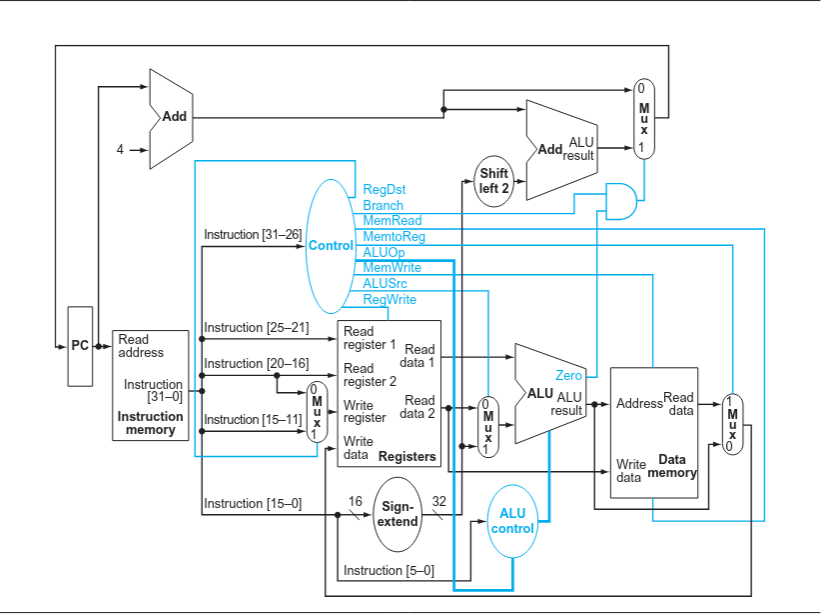
\includegraphics[width=\paperwidth]{datapath.png}}
%     \caption{Description of your full-width image}
% \end{figure}

\begin{landscape}
\begin{table}[h]
\renewcommand{\arraystretch}{1.4}
\setlength{\tabcolsep}{5.5pt}
\hspace{-3.8cm}
\makebox[\textwidth][l]{
\begin{tabular}{|c|c|c|c|c|c|c|c|c|c|c|c|}
\hline
\textbf{Opcode} & \textbf{Instruction} & \textbf{RegDst} & \textbf{Jump} & \textbf{Brancheq} & \textbf{Branchneq} & \textbf{MemRead} & \textbf{MemtoReg} & \textbf{MemWrite} & \textbf{ALUSrc} & \textbf{RegWrite} &\textbf{ALUCtrl} \\
\hline
0  & lw   & 0 & 0 & 0 & 0 & 1 & 1 & 0 & 1 & 1 & 010 (ADD) \\ \hline
1  & bneq & X & 0 & 0 & 1 & 0 & X & 0 & 0 & 0 & 011 (SUB) \\ \hline
2  & subi & 0 & 0 & 0 & 0 & 0 & 0 & 0 & 1 & 1 & 011 (SUB) \\ \hline
3  & beq  & X & 0 & 1 & 0 & 0 & X & 0 & 0 & 0 & 011 (SUB) \\ \hline
4  & j    & X & 1 & 0 & 0 & 0 & X & 0 & X & 0 & ---       \\ \hline
5  & addi & 0 & 0 & 0 & 0 & 0 & 0 & 0 & 1 & 1 & 010 (ADD) \\ \hline
6  & sw   & X & 0 & 0 & 0 & 0 & X & 1 & 1 & 0 & 010 (ADD) \\ \hline
7  & or   & 1 & 0 & 0 & 0 & 0 & 0 & 0 & 0 & 1 & 001 (OR)  \\ \hline
8  & add  & 1 & 0 & 0 & 0 & 0 & 0 & 0 & 0 & 1 & 010 (ADD) \\ \hline
9  & and  & 1 & 0 & 0 & 0 & 0 & 0 & 0 & 0 & 1 & 000 (AND) \\ \hline
10 & ori  & 0 & 0 & 0 & 0 & 0 & 0 & 0 & 1 & 1 & 001 (OR)  \\ \hline
11 & nor  & 1 & 0 & 0 & 0 & 0 & 0 & 0 & 0 & 1 & 100 (NOR) \\ \hline
12 & andi & 0 & 0 & 0 & 0 & 0 & 0 & 0 & 1 & 1 & 000 (AND) \\ \hline
13 & sub  & 1 & 0 & 0 & 0 & 0 & 0 & 0 & 0 & 1 & 011 (SUB) \\ \hline
14 & sll  & 0 & 0 & 0 & 0 & 0 & 0 & 0 & 1 & 1 & 101 (SHIFT LEFT)  \\ \hline
15 & srl  & 0 & 0 & 0 & 0 & 0 & 0 & 0 & 1 & 1 & 111 (SHIFT RIGHT) \\ \hline
\end{tabular}
}
\caption{Control Signals and ALU Control Lines for Each Instruction}
\end{table}
\end{landscape}
\end{document}